
\documentclass[10pt,a4paper]{article}

% Om het totaal aantal pagina's te tellen
\usepackage{lastpage}
\usepackage{graphicx}

% Om de marges aan te passen
\usepackage[left=2cm,right=2cm,top=2cm,bottom=2cm]{geometry}

% Voor headers en footers
\usepackage{fancyhdr}
\pagestyle{fancy}

\lhead{Giuseppe Callari and Xavier Go\'as Aguililla}
\rhead{\thepage /\pageref{LastPage}}

\lfoot{Assignment}
\cfoot{Computer Networks}
\rfoot{Network Simulation}

\renewcommand{\headrulewidth}{0.4pt}
\renewcommand{\footrulewidth}{0.4pt}

\begin{document}
\begin{titlepage}
\thispagestyle{empty}
\newcommand{\HRule}{\rule{\linewidth}{0.5mm}}
\center
\textsc{\LARGE KU Leuven}\\[1.5cm]
\vfill

% \HRule \\[0.4cm]
{ \Huge \bfseries Network simulation with NS/2}\\[0.4cm]
% \HRule \\[1.5cm]
\vfill

\begin{minipage}{0.4\textwidth}
\begin{flushleft} \large
\emph{Authors:}\\
Giuseppe \textsc{Callari} (r0301006)\\
Xavier \textsc{Go\'as Aguililla} (s0201506)
\end{flushleft}
\end{minipage}
~
\begin{minipage}{0.4\textwidth}
\begin{flushright} \large
\textsc{\large Computer networks [G0Q43A]}\\[0.5cm]
\emph{Professor:} \\
prof. dr. Daniel \textsc{Hughes}\\
\emph{Assistant:} \\
dr. Nelson \textsc{Matthys}\\
\end{flushright}
\end{minipage}\\[4cm]

{\large May 2nd, 2014}\\[3cm]
\vfill

\end{titlepage}


\section{Exercise 1}
\subsection{Question 1}
In figure \ref{fig:lala} we can clearly see the difference between the
scenario with both an uploader and a downloader and that without an
uploader. In the scenario with an uploader, around the time the upload
starts (3.0s), the throughput for the downloader drops drastically. In
the scenario without an uploader, indicated in green, the throughput
of the connection remains roughly constant.

\begin{figure}[p]
    \centering
    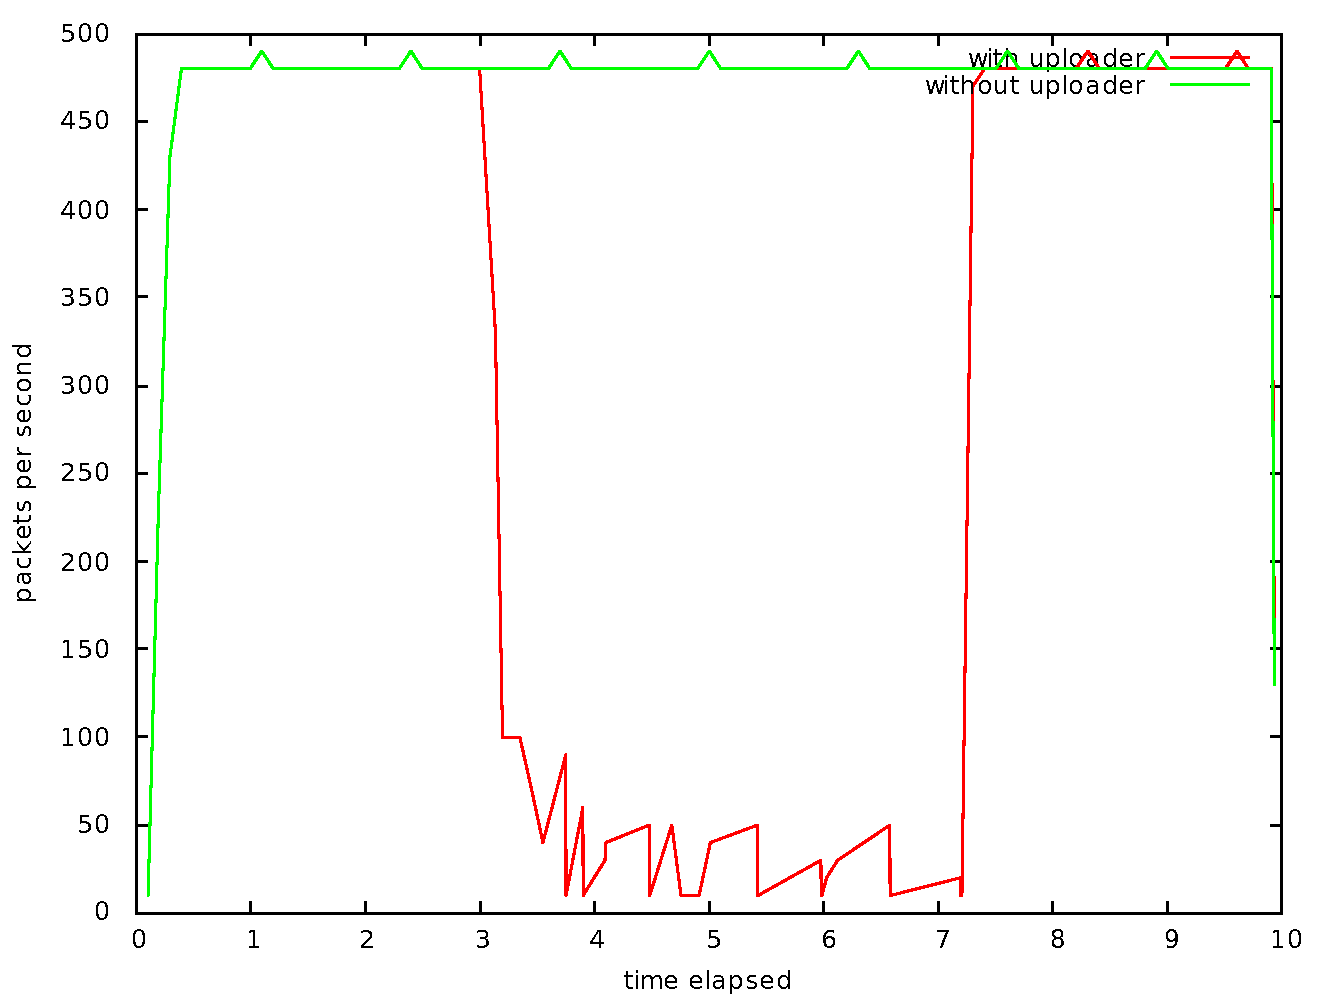
\includegraphics[width=\textwidth]{../part1/q1/plots/1.pdf}
    \caption{Download throughput compared}
    \label{fig:lala}
\end{figure}

\subsection{Question 2}
In figure \ref{fig:combined1} we see both the upload and download
throughput on the same graph; we can clearly see the aforementioned
drop in download speed at the moment the upload over CBR starts.

\begin{figure}[p]
    \centering
    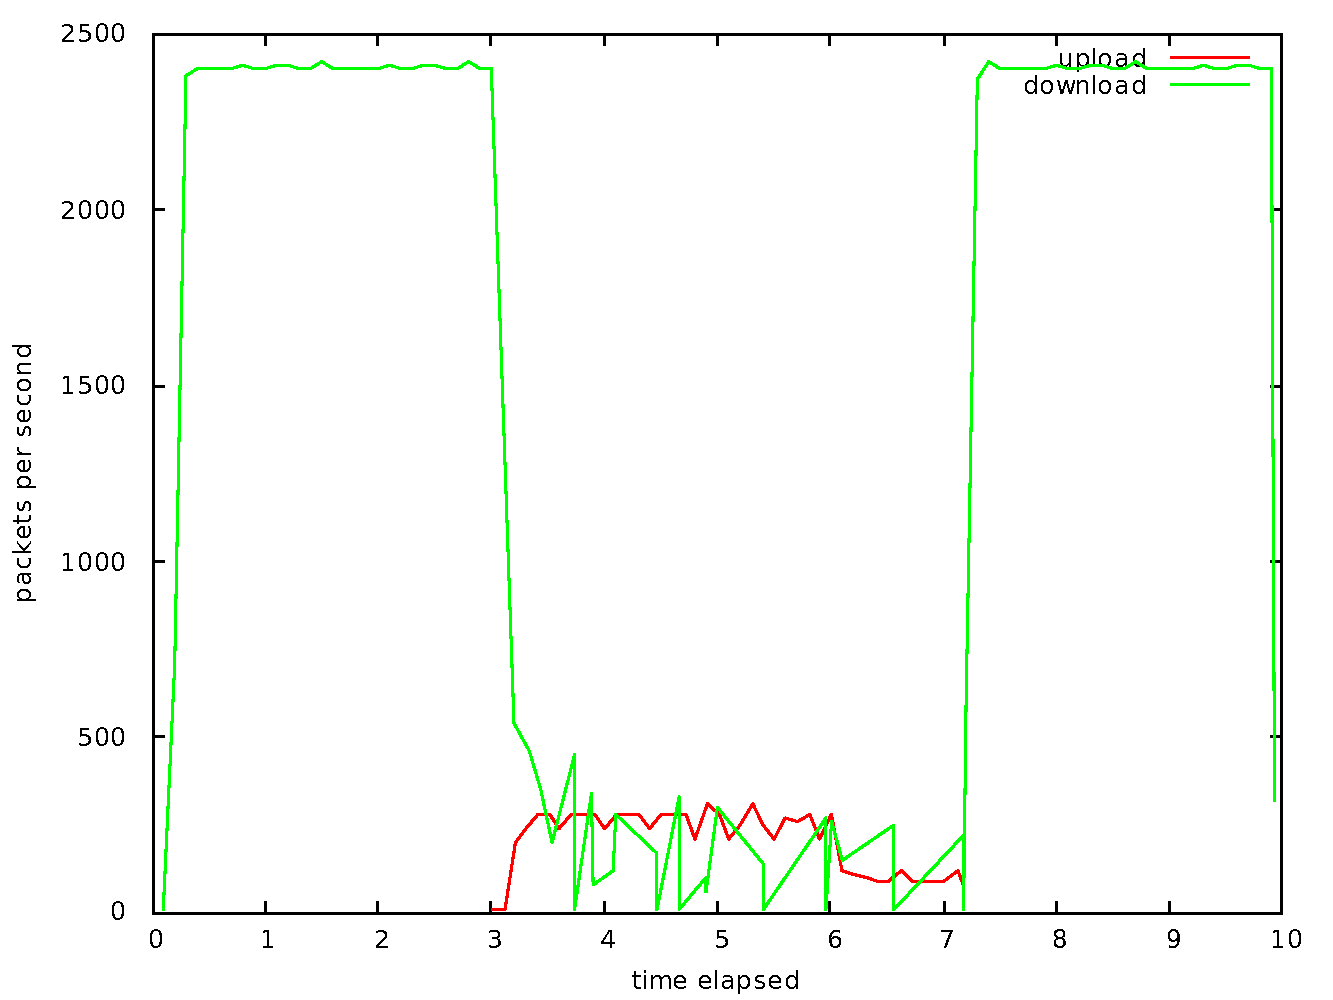
\includegraphics[width=\textwidth]{../part1/q2/plots/2.pdf}
    \caption{Upload and download throughput}
    \label{fig:combined1}
\end{figure}
\subsection{Question 3}

We expect performance for CBR to be excellent, since a certain amount
of bandwidth is always guaranteed for the upload connection. This does
imply that the upload connection has a certain privilege over the
download connection; to ensure this, we could tell the router to drop
downstream packets rather than upstream packets. This would result in
increased packet loss for the download connection, especially if we
would run multiple upload connections at the same time.

\subsection{Question 4}

We can see in figures \ref{fig:down_limited} and \ref{fig:up_limited} that
both the bridled and unbridled connection show similar patterns but
differ at the tail end of the speed drop from 3.0s on. At 6.0s the CBR
upload is stopped, but not all packets have been transferred yet due
to packet loss.

The connection layer ensures these lost packets still arrive at their
destination. To do this, the TCP connection persists while not all
packets have arrived at their destination. Looking at figure
\ref{fig:up_limited}, we see that the TCP upstream connection persists
longer in the situation with the limited bandwidth. The packets
transferred while the connection persists take up a certain amount of
bandwidth. Only around the 9.5 second mark are all the packets
transferred, and in figure \ref{fig:down_limited} we can see that the FTP
download is negatively affected by this transfer: the throughput is
very low until the 9.5 second mark.

\begin{figure}[p]
    \centering
    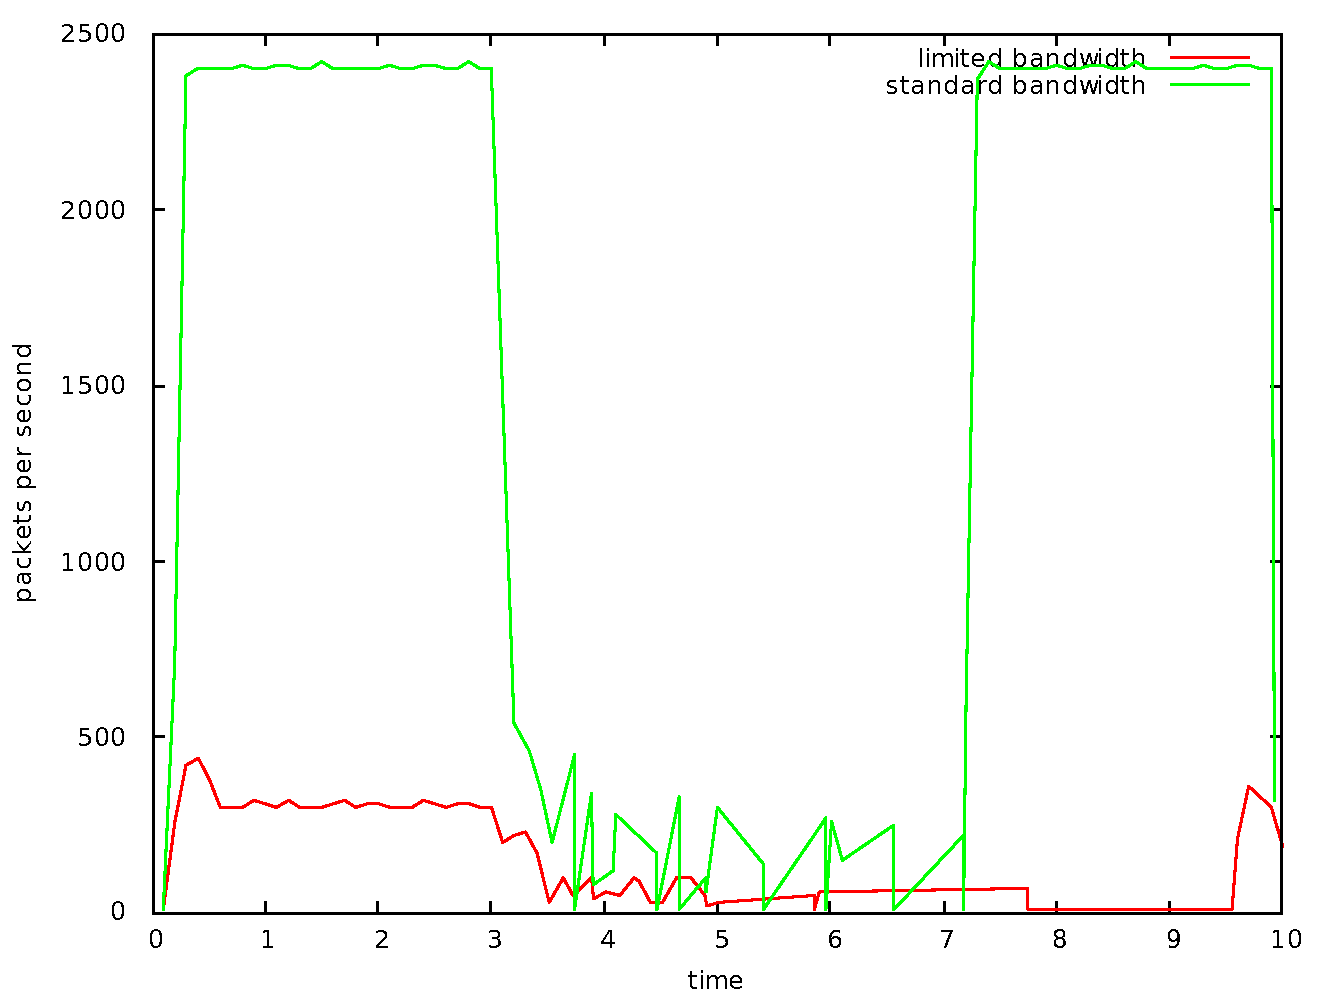
\includegraphics[width=\textwidth]{../part1/q4/plots/4-down.pdf}
    \caption{Download throughput}
    \label{fig:down_limited}
\end{figure}

\begin{figure}[p]
    \centering
    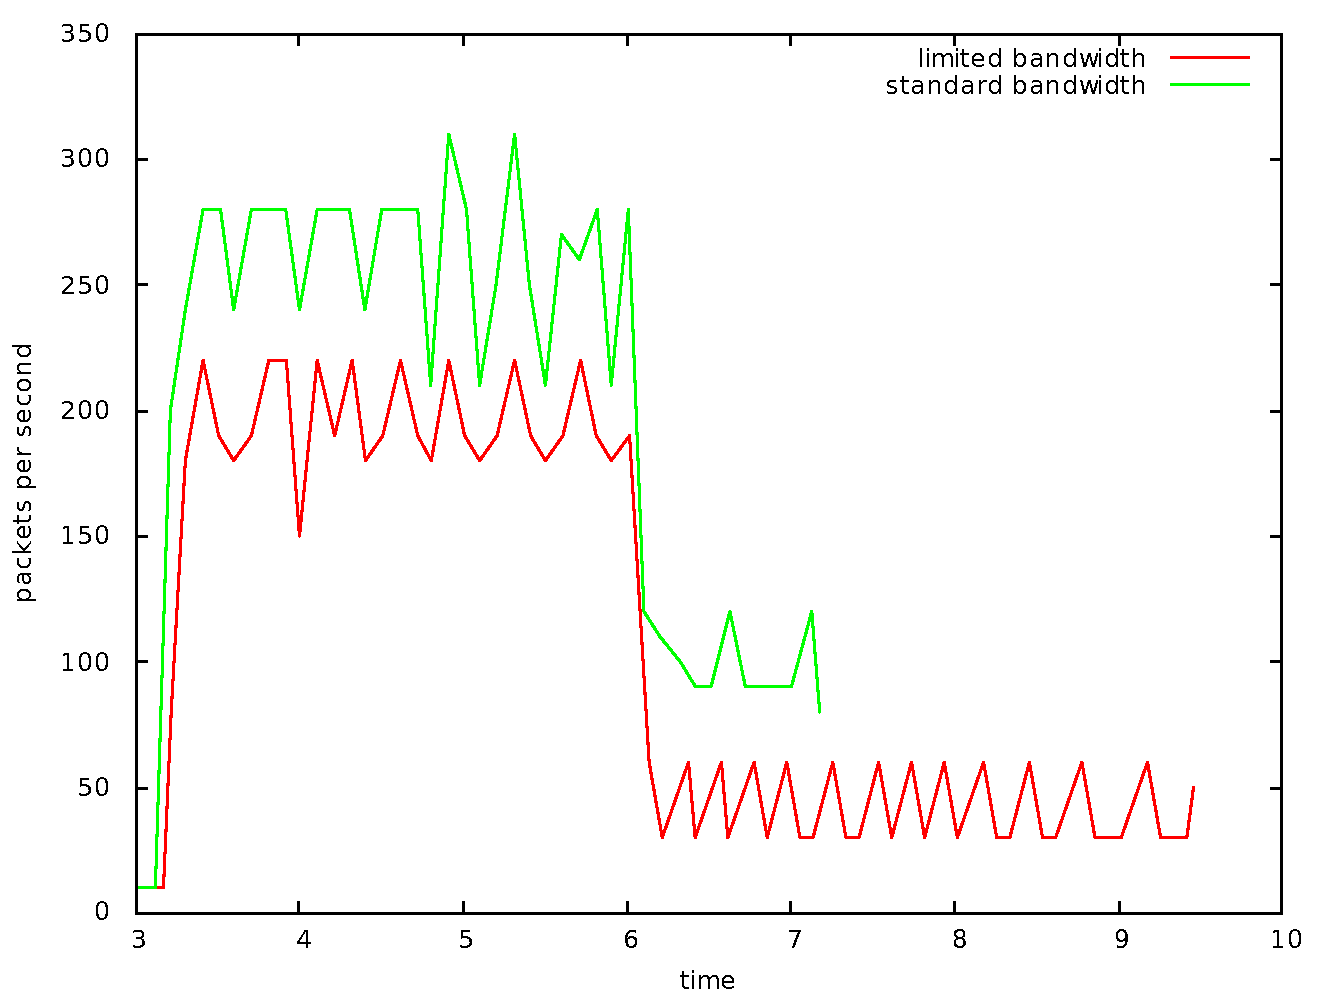
\includegraphics[width=\textwidth]{../part1/q4/plots/4-up.pdf}
    \caption{Upload throughput}
    \label{fig:up_limited}
\end{figure}

\subsection{Question 5}

When we impose a fixed bitrate on the CBR connection, we ensure that
this connection never takes more than its preallocated share of
bandwidth. Thus, when we allocate a small percentage of the total
connection bandwidth, we ensure that other connections on the same
link will not suffer from greatly limited performance, since TCP will
not allocate more bandwidth than this fixed rate. TCP can then
dynamically allocate bandwidth to other connections.

% observations from simulation %

\subsection{Question 6}

\subsubsection{Question 6-1}
A naive response would be to say that we expect performance to stay
the same, since we have ten times the bandwidth for ten times the
users. In actuality, this is not true. Consider the output of a
simulation we made for this scenario.

We can clearly see that all transfers have very variable throughput.

\subsubsection{Question 6-2}

\section{Exercise 2}
\subsection{Question 1}
\subsection{Question 2}
\subsection{Question 3}
\subsection{Question 4}

\end{document}